% Numbers and data-dependent verdicts are macros from generated/results.tex, written by
% reports/mid_submission/build_results.py from the Ada C-v1 run; its decision rules are fixed there.
\begin{abstract}
We investigate whether entropy-triggered boundaries in the Byte Latent Transformer (BLT) align with syntactic constituent starts beyond a density-matched null. Project ESCAPE compares Python, C++, and English prose. We restore the patcher's 512-byte sliding window, extract entropies for all \nSamples{} files, freeze the matching tolerance on a calibration split, and score the held-out split with one-to-one matching against \nPerm{} permutations of each file's own patch lengths. Held-out start F1 \POneAll{} (Python \FonePy{} vs.\ \FoneNullPy{}; C++ \FoneCpp{} vs.\ \FoneNullCpp{}; English \FoneEn{} vs.\ \FoneNullEn{}). Against the strongest structure-blind baseline (indentation or word starts), however, BLT \RTwoAll{}. By constituent type, forced-opener constructs such as \texttt{if} and \texttt{def} align more strongly than open-ended ones, contrary to our prediction. Under injected code noise, alignment degrades only slightly, while noise lowers bytes per patch. Entropy is a surface statistic, and none of these results is evidence of semantic understanding.
\end{abstract}

\section{Introduction}
Byte-level models remove a fixed subword vocabulary, but computation still needs to be allocated across long input sequences. BLT groups bytes into variable-length patches using a small next-byte entropy model \citep{pagnoni-etal-2025-byte}. A boundary at the start of a syntactic constituent could indicate that this allocation tracks structure. Rare identifiers, word starts, and formatting can also induce boundaries, so proximity alone cannot distinguish these explanations.

ESCAPE asks whether entropy-triggered boundaries align with constituent starts more than a null with the same patch-length distribution and boundary count (P1). We also ask whether they align more at starts than at ends (P2), more in code than in prose (P3), and less for constructs whose opening is forced than for open-ended ones (P4). A further question is whether any extra patching near memory-unsafe C++ persists after identifier controls. These are empirical hypotheses: entropy bounds branching ($H\le\log B$) but is neither a grammatical branching factor nor a measure of program semantics. This report gives held-out results for P1--P4 against both the null and structure-blind baselines, span IoU as a secondary metric, and robustness to code noise (Objective 4).

\section{Background and Related Work}
BLT dynamically segments byte sequences so that expensive latent computation operates over patches \citep{pagnoni-etal-2025-byte}. Our analysis concerns its entropy patcher, not downstream generation accuracy. ByT5 demonstrates an alternative byte-level modeling approach \citep{xue-etal-2022-byt5}; neither architecture by itself establishes correspondence between computational units and syntax.

We use code AST starts and predicted English constituent starts as external structural references. Python samples come from CodeSearchNet \citep{husain2019codesearchnet}, and C++ uses a subset of The Stack \citep{kocetkov2022stack}. English paragraphs come from WikiText-103 \citep{merity2017pointer} and are parsed with benepar \citep{kitaev-klein-2018-constituency}. These reference structures differ in granularity and reliability, motivating language-specific calibration and reporting.

\section{Evaluation Protocol}
\label{sec:protocol}
\paragraph{Byte contract and metric.} All positions are frozen UTF-8 byte offsets; spans are half-open. Versioned JSONL interfaces carry sample metadata and hashes, patcher outputs, ground-truth nodes, and region annotations. Validators check joins, hashes, lengths, patch tiling, and entropy coverage. Entropy at byte $i$ is the model's global Shannon entropy
\begin{equation}
H_i=-\sum_{v\in\mathcal{V}}p_\theta(v\mid x_{<i})\log p_\theta(v\mid x_{<i})
\end{equation}
over its 260 output symbols, in nats. Predictions are interior boundaries labelled \texttt{entropy}. Targets are unique starts of eligible, non-wrapper, positive-length nodes, excluding byte zero and file end. Maximum-cardinality one-to-one matching pairs predictions and targets within $k$ bytes. With $T$ matches, $P$ predictions and $G$ targets, precision is $T/P$, recall $T/G$ and F1 $2T/(P+G)$, pooled across files. Ends are scored the same way.

\paragraph{Frozen tolerance and null.} Each language is split at the file level by a seeded SHA256 rank: 20\% calibration, 80\% test. Only calibration files evaluate $k\in\{0,1,2,4,8\}$, and we choose the $k$ maximizing the median per-file F1 margin over the null, ties to the smaller $k$. The hashed record is verified at scoring, and there is no test-time override. For each file, $H_0$ shuffles the (length, termination) pairs of all patches except the last, which stays in place so that file end never becomes a scored boundary, and rebuilds the endpoints. This preserves file length, the patch-length multiset and the number of entropy boundaries. Each of \nPerm{} seeded permutations shuffles every test file independently. We report the null mean, the one-sided permutation value, and paired file-bootstrap 95\% intervals (\nBoot{} replicates).

\paragraph{Structure-blind baselines.} Under the same targets, $k$ and matching, we score boundaries after every newline, at indentation changes, and at every word start. A structural reading requires BLT to beat these, since most code constituents begin after a line break and most prose constituents begin at a word. We report BLT minus baseline F1 with a paired file bootstrap.

\section{Data and Checkpoint}
The frozen manifest has \nSamples{} samples: 8{,}000 Python functions (CodeSearchNet), 8{,}000 C++ files (The Stack, smol) and 300 English paragraphs (WikiText-103). All bytes were restored and verified against stored hashes. Calibration used \nCalPy{}/\nCalCpp{}/\nCalEn{} files and testing \nTestPy{}/\nTestCpp{}/\nTestEn{} (Python/C++/English). The selected tolerances were $k=\kPy$, $\kCpp$ and $\kEn$.

We use the Hugging Face conversion \texttt{itazap/blt-1b-hf} (revision \texttt{91aa6b8e}), loading only its 99.5M-parameter patcher. It runs in float32 with threshold 1.3354 nats, no length cap, and the reference 512-token sliding window and 8{,}192-token chunks, which the port omits. Extraction ran on four RTX 2080 Ti GPUs of the IIIT-H Ada cluster, and all \nExtracted{} files completed with consistent artifacts. Six of eight original fidelity gates passed; two failed (tokenizer EOS and a random-byte threshold). The amended checks, which use the actual BOS-plus-byte input and require over 90\% random-byte boundary density, pass. Rerun on the cluster's software stack, the amended gate set \FidelityAda{}. This establishes agreement with an independent reference implementation, not identity with the original weights.

\section{Results}
\TableMain
\paragraph{P1: alignment beyond the null.} Table~\ref{tab:main} gives held-out start alignment. The F1 margin over $H_0$ is \MarginPy{} \MarginCIPy{} in Python, \MarginCpp{} \MarginCICpp{} in C++ and \MarginEn{} \MarginCIEn{} in English. Precision/recall are \PrecPy{}/\RecPy{}, \PrecCpp{}/\RecCpp{} and \PrecEn{}/\RecEn{}. A sufficient-but-not-necessary mechanism predicts precision above recall. Precision \PrecRecAll{}. BLT proposes many more boundaries than there are targets, so most boundaries fall away from constituent starts.

\TableBaselines
\paragraph{Baselines.} The strongest structure-blind proposer is the \StrongestPy{} baseline for Python (F1 \StrongestFonePy{}), the \StrongestCpp{} baseline for C++ (\StrongestFoneCpp{}) and the \StrongestEn{} baseline for English (\StrongestFoneEn{}). BLT \RTwoAll{} (Python \VsBasePy{} \VsBaseCIPy{}; C++ \VsBaseCpp{} \VsBaseCICpp{}; English \VsBaseEn{} \VsBaseCIEn{}). With the frozen $k=0$, the newline baseline scores near zero: an indented statement starts after its indentation, not at the byte after the newline, and each English sample is a single paragraph. A margin over $H_0$ that does not survive this comparison indicates line or word segmentation rather than syntactic structure.

\paragraph{P2 and P3.} The start margin \PTwoAll{} (end margins \EndMarginPy{}, \EndMarginCpp{} and \EndMarginEn{} for Python, C++ and English). These two margins share predictions and are compared descriptively. Pooled by domain, the code margin (\MarginCode{}) is \PThreeCmp{} the prose margin (\MarginProse{}), so P3 is not supported; in English, BLT also falls short of the word-start baseline (Table~\ref{tab:baselines}). Mean bytes per patch are \BppPy{}, \BppCpp{} and \BppEn{} (Python, C++, English), with mean within-file BPP variances \BppVarPy{}, \BppVarCpp{} and \BppVarEn{}.

\TableTypes
\paragraph{P4 and depth.} Averaged over types, the recall margin over $H_0$ for forced-opener constructs is \DetMarginPy{} in Python and \DetMarginCpp{} in C++, against \OpenMarginPy{} and \OpenMarginCpp{} for open-ended ones (Table~\ref{tab:types}). The forced-opener margin \PFourAll{}, so the data \PFourSupported{} P4 as stated. One reading is that a start boundary precedes the keyword, where the choice of statement is still open; the forcing we predicted applies to the bytes after it, which starts do not measure. Figure~\ref{fig:depth} shows the start recall margin by tree depth.

\begin{figure}[t]
\centering
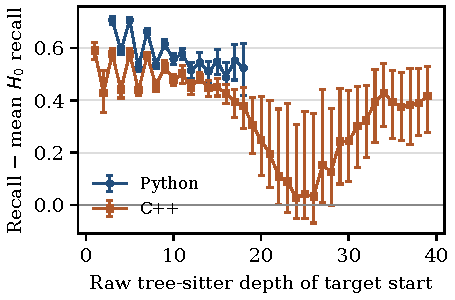
\includegraphics[width=\columnwidth]{generated/depth_margin.pdf}
\caption{Held-out start recall minus mean $H_0$ recall by raw tree-sitter depth, for strata with at least 200 target starts. Recall is used because all strata share one prediction set. Raw depth is not comparable across languages. Whiskers are file-bootstrap 95\% intervals of recall.}
\label{fig:depth}
\end{figure}

\TableIoU
\paragraph{Secondary: span IoU.} For each unique constituent span we take its best IoU with a single patch (Table~\ref{tab:iou}). BLT exceeds the null by \IouVsNullPy{} \IouVsNullCIPy{} in Python, \IouVsNullCpp{} \IouVsNullCICpp{} in C++ and \IouVsNullEn{} \IouVsNullCIEn{} in English. In code, line segmentation matches spans far better (\IouLinePy{} and \IouLineCpp{}). Patches are much shorter than most constituents, so IoU understates alignment by design; it is secondary to start P/R.

\TableOFour
\paragraph{Objective 4: robustness to code noise.} On \OFourFiles{} held-out files per language we inject the four noise types of our proposal, each on its own: missing statement semicolons (C++), a one-space indentation change on \OFourRate{} of lines, consistent camelCase$\leftrightarrow$snake\_case renaming of \OFourCaseRate{} of convertible identifiers, and adjacent-letter swaps in \OFourRate{} of keywords. Targets are the clean constituents mapped to their noised offsets, so we measure whether boundaries still track the intended structure. The margin over $H_0$ is \OFourCleanPy{} (Python) and \OFourCleanCpp{} (C++) on clean code (Table~\ref{tab:o4}). The largest drop comes from \OFourWorstPy{} noise in Python (\OFourWorstDmPy{} \OFourWorstDmCIPy{}) and \OFourWorstCpp{} noise in C++ (\OFourWorstDmCpp{} \OFourWorstDmCICpp{}); every noised margin stays at or above \OFourMinMarginPy{} and \OFourMinMarginCpp{}. Patching thus degrades gracefully rather than failing. Keyword typos change BPP most (\OFourDbppPyTypo{} and \OFourDbppCppTypo{} bytes per patch), since misspelled keywords are unpredictable and receive more patches.

\section{Remaining Work and Conclusion}
BLT's entropy boundaries sit at constituent starts far more often than its own patch lengths would by chance. Relative to the strongest structure-blind baseline, however, BLT \RTwoAll{}. Any structural claim must therefore be made relative to line and word segmentation, not the null alone.
For the final submission we will review the memory-unsafe-region regression (O5) and its region labels, and test the P4 reversal against byte positions after the opening keyword. We will also vary the noise rates for Objective 4. The measurement pipeline, the frozen calibration and the held-out scores reported here are fixed inputs to that work.

\section*{Limitations}
The checkpoint is a third-party conversion, and the sliding window was restored by us. English targets come from predicted parses, and the English paragraphs were inspected in an earlier exploratory analysis before this protocol was frozen. About 28\% of C++ files trigger parser error recovery; they are included. Python samples are functions that may share repositories, so file bootstraps need not generalize across projects. The null fixes the final patch. Word and newline baselines are deterministic and not density matched. Objective 4 uses one noise rate per type and 1{,}000 null permutations per file, and span IoU uses 100.

\section*{Ethical Considerations}
The project analyzes existing text and source code without executing corpus programs. Dataset provenance and licenses accompany restored inputs; CodeSearchNet carries no per-file license.

\bibliography{references}
\bibliographystyle{acl_natbib}
